% +------------------------------------------------------------------------+
% | Reference manual page: Subdivision_surfaces_3.tex
% +------------------------------------------------------------------------+
% | 03/01/2005   Le-Jeng Andy Shiue
% | Package: Subdivision_surface_3
% | 
\RCSdef{\RCSSubdivisionRev}{$Revision$}
\RCSdefDate{\RCSSubdivisionDate}{$Date$}
% +------------------------------------------------------------------------+

\ccRefPageBegin

%%RefPage: end of header, begin of main body
% +------------------------------------------------------------------------+


\begin{ccRefClass}{PQQ_stencil}

\ccDefinition

A stencil maps an input submesh to a point on the refined 
mesh. \ccClassTemplateName\ defines the policy interface of 
stencils of the PQQ refinement. \ccClassTemplateName\ does not
realize the geometry masks of a specific subdivision schemes.
\ccClassTemplateName\ also defines the policy interface 
of stencils of PTQ and $\sqrt{3}$ refinement.

%% \begin{ccTexOnly}
%%     \vspace{-7mm}
%%     \begin{center}
%%       \parbox{0.4\textwidth}{%
%%         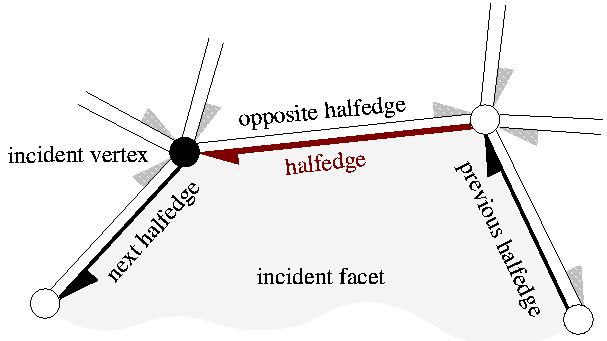
\includegraphics[width=0.4\textwidth]{Polyhedron_ref/fig/halfedge}%
%%       }
%%     \end{center}
%%     \vspace{-5mm}
%% \end{ccTexOnly}

%% \begin{ccHtmlOnly}
%%     <CENTER>
%%     <A HREF="fig/halfedge.gif">
%%         <img src="fig/halfedge_small.gif" alt="Halfedge Diagram"></A><P>
%%     </CENTER>
%% \end{ccHtmlOnly}

\ccInclude{CGAL/Subdivision_surfaces_rules_3.h}

\ccParameters

The full template declaration of \ccClassTemplateName\ states one
template parameter:

\begin{tabbing}
\ccc{template <} \=\ccc{class _Poly>}\\
     \ccc{class PQQ_stencil;}
\end{tabbing}
   
The \ccc{_Poly} parameter requires a model of 
the \ccc{Polyhedron_3} concept as argument. \ccc{Point_3} 
is required to be typedefined in \ccc{_Poly}.

%% \ccTypes

%% \ccNestedType{Traits}{traits class selected for \ccc{PolyhedronTraits_3}.}
%% \ccGlue
%% \ccNestedType{Items}{items class selected for \ccc{PolyhedronItems_3}.}
%% \ccGlue



%% % +-----------------------------------+
%% \begin{ccAdvanced}
%% \ccHeading{Types for Tagging Optional Features}

%% \ccNestedType{Supports_facet_plane}{\ccc{Facet::plane()}.}
%% \ccGlue
%% \ccNestedType{Supports_removal}{supports removal of individual elements.}

%% \end{ccAdvanced}

\ccCreation
%\ccCreationVariable{P}

%\ccClassTemplateName\ is a functor of the three geometry stencils for
%subdivision surfaces based on the PQQ refinement. 
Default constructors are generated by the compiler.


% +-----------------------------------+
\ccHeading{Stencil Policies}
\ccThree{}{}{}

\ccMethod{void facet_node(Facet_handle f, Point& pt)}
{define the access interface of the facet-node stencil. 
\ccc{pt} is semantically smoothed by averaging points of the
neighborhood of \ccc{f}.
Override this function to support geometry masks for subdivisions 
based on PQQ and $\sqrt{3}$ refinement.} 

\ccMethod{void edge_node(Edge_handle e, Point& pt)}
{define the access interface of the edge-node stencil. 
\ccc{pt} is semantically smoothed by averaging points of 
the neighborhood of \ccc{e}.
Override this function to support geometry masks for subdivisions 
based on PQQ and PTQ refinement.} 

\ccMethod{void vertex_node(Vertex_handle v, Point& pt)}
{define the access interface of the vertex-node stencil.
\ccc{pt} is semantically smoothed by averaging points of 
the neighborhood of \ccc{v}.
Override this function to support geometry masks for subdivisions 
based on PQQ, PTQ and $\sqrt{3}$ refinement.} 


%% \begin{ccTexOnly}
%%     \begin{center}
%%       \parbox{0.636\textwidth}{%
%%           \includegraphics[width=0.636\textwidth]%
%%               {Polyhedron_ref/fig/euler_loop}%
%%       }
%%     \end{center}
%% \end{ccTexOnly}
%% \begin{ccHtmlOnly}
%%     <CENTER>
%%     <img src="fig/euler_loop.gif" alt="Euler Operator: Loop"><P>
%%     </CENTER>
%% \end{ccHtmlOnly}


\ccSeeAlso

\ccRefIdfierPage{CGAL::Subdivision_surfaces_3}\\
\ccRefIdfierPage{CGAL::DQQ_stencil}\\
\ccRefIdfierPage{CGAL::Linear_stencil}\\
\ccRefIdfierPage{CGAL::CatmullClark_stencil}\\
\ccRefIdfierPage{CGAL::Loop_stencil}\\
\ccRefIdfierPage{CGAL::Sqrt3_stencil}\\

%\ccExample
%This example program instantiates a polyhedron using the default
%traits class and creates a tetrahedron.
%\ccIncludeExampleCode{Polyhedron/polyhedron_prog_simple.C}

\end{ccRefClass}

% +------------------------------------------------------------------------+
%%RefPage: end of main body, begin of footer
\ccRefPageEnd
% EOF



% +------------------------------------------------------------------------+
% +------------------------------------------------------------------------+
\ccRefPageBegin

%%RefPage: end of header, begin of main body
% +------------------------------------------------------------------------+

\begin{ccRefClass}{DQQ_stencil}

\ccDefinition

A stencil maps an input submesh to a point on the refined 
mesh. \ccClassTemplateName\ defines the policy interface of 
stencils of the DQQ refinement. \ccClassTemplateName\ does not
realize the geometry masks of a specific subdivision schemes.

\ccInclude{CGAL/Subdivision_surfaces_rules_3.h}

\ccParameters

The full template declaration of \ccClassTemplateName\ states one
template parameter:

\begin{tabbing}
\ccc{template <} \=\ccc{class _Poly>}\\
     \ccc{class DQQ_stencil;}
\end{tabbing}
   
The \ccc{_Poly} parameter requires requires a model of 
the \ccc{Polyhedron_3} concept as argument. \ccc{Point_3} 
is required to be typedefined in \ccc{_Poly}.

\ccCreation
%\ccCreationVariable{P}

Default constructors are generated by the compiler.


% +-----------------------------------+
\ccHeading{Stencil Policies}
\ccThree{}{}{}

\ccMethod{void corner_node(Halfedge_handle he, Point& pt)}
{define the access interface of the corner-node stencil 
of the DQQ refinement. 
\ccc{pt} is semantically smoothed by averaging points on 
the facet of \ccc{he}. \ccc{he} points to the vertex 
which usually has the dominate mask weight.}

\ccSeeAlso

\ccRefIdfierPage{CGAL::Subdivision_surfaces_3}\\
\ccRefIdfierPage{CGAL::PQQ_stencil}\\
\ccRefIdfierPage{CGAL::DooSabin_stencil}\\

\end{ccRefClass}

% +------------------------------------------------------------------------+
%%RefPage: end of main body, begin of footer
\ccRefPageEnd
% EOF
% +------------------------------------------------------------------------+



% +------------------------------------------------------------------------+
% +------------------------------------------------------------------------+
\begin{ccRefClass}{Linear_stencil}

\ccDefinition

\ccClassTemplateName , derived the policy interface of 
\ccc{PQQ_Stencil}, realizes the geometry masks as linear 
averaging of points collected from the input submesh.

\ccInclude{CGAL/Subdivision_surfaces_rules_3.h}

\ccParameters

The full template declaration of \ccClassTemplateName\ states one
template parameter:

\begin{tabbing}
\ccc{template <} \=\ccc{class _Poly>}\\
     \ccc{class Linear_stencil;}
\end{tabbing}
   
The \ccc{_Poly} parameter requires requires a model of 
the \ccc{Polyhedron_3} concept as argument. 
\ccc{Point_3} is required to be typedefined in \ccc{_Poly}.

\ccCreation
%\ccCreationVariable{P}

Default constructors are generated by the compiler.


% +-----------------------------------+
\ccHeading{Stencil Policies}
\ccThree{}{}{}

\ccMethod{void facet_node(Facet_handle f, Point& pt)}
{assign the centroid of \ccc{f} to \ccc{pt}.}

\ccMethod{void edge_node(Edge_handle e, Point& pt)}
{assign the mid-point of \ccc{e} to \ccc{pt}}

\ccMethod{void vertex_node(Vertex_handle v, Point& pt)}
{assign the point on \ccc{v} to \ccc{pt}}

\ccSeeAlso

\ccRefIdfierPage{CGAL::Subdivision_surfaces_3}\\
\ccRefIdfierPage{CGAL::PQQ_stencil}\\
\ccRefIdfierPage{CGAL::CatmullClark_stencil}\\
\ccRefIdfierPage{CGAL::Loop_stencil}\\
\ccRefIdfierPage{CGAL::Sqrt3_stencil}\\

\end{ccRefClass}

% +------------------------------------------------------------------------+
%%RefPage: end of main body, begin of footer
\ccRefPageEnd
% EOF
% +------------------------------------------------------------------------+



% +------------------------------------------------------------------------+
% +------------------------------------------------------------------------+
\begin{ccRefClass}{CatmullClark_stencil}

\ccDefinition

\ccClassTemplateName , derived from the \ccc{Linear_stencil},
implements the geometry masks of Catmull-Clark subdivision. 

\ccInclude{CGAL/Subdivision_surfaces_rules_3.h}

\ccParameters

The full template declaration of \ccClassTemplateName\ states one
template parameter:

\begin{tabbing}
\ccc{template <} \=\ccc{class _Poly>}\\
     \ccc{class Linear_stencil;}
\end{tabbing}
   
The \ccc{_Poly} parameter requires requires a model of 
the \ccc{Polyhedron_3} concept as argument. 
\ccc{Point_3} is required to be typedefined in \ccc{_Poly}.

\ccCreation
%\ccCreationVariable{P}

Default constructors are generated by the compiler.

% +-----------------------------------+
\ccHeading{Stencil Policies}
\ccThree{}{}{}

\ccMethod{void facet_node(Facet_handle f, Point& pt)}
{compute the Catmull-Clark facet-point on \ccc{f}, 
and assign the smoothed point to \ccc{pt}.}

\ccMethod{void edge_node(Edge_handle e, Point& pt)}
{compute the Catmull-Clark edge-point on the 1-ring
of \ccc{e}, and assign the smoothed point to \ccc{pt}.}

\ccMethod{void vertex_node(Vertex_handle v, Point& pt)}
{compute the Catmull-Clark vertex-point on the 
1-ring of \ccc{v}, and assign the smoothed point to \ccc{pt}.}


\ccSeeAlso

\ccRefIdfierPage{CGAL::Subdivision_surfaces_3}\\
\ccRefIdfierPage{CGAL::PQQ_stencil}\\
\ccRefIdfierPage{CGAL::Linear_stencil}\\

\end{ccRefClass}

% +------------------------------------------------------------------------+
%%RefPage: end of main body, begin of footer
\ccRefPageEnd
% EOF
% +------------------------------------------------------------------------+


% +------------------------------------------------------------------------+
% +------------------------------------------------------------------------+
\begin{ccRefClass}{Loop_stencil}

\ccDefinition

\ccClassTemplateName , derived from \ccc{PQQ_stencil}, 
defines the geometry masks of Loop subdivision. 

\ccInclude{CGAL/Subdivision_surfaces_rules_3.h}

\ccParameters

The full template declaration of \ccClassTemplateName\ states one
template parameter:

\begin{tabbing}
\ccc{template <} \=\ccc{class _Poly>}\\
     \ccc{class Linear_stencil;}
\end{tabbing}
   
The \ccc{_Poly} parameter requires requires a model of 
the \ccc{Polyhedron_3} concept as argument. 
\ccc{Point_3} is required to be typedefined in \ccc{_Poly}.

\ccCreation
%\ccCreationVariable{P}

Default constructors are generated by the compiler.

% +-----------------------------------+
\ccHeading{Stencil Policies}
\ccThree{}{}{}

\ccMethod{void edge_node(Edge_handle e, Point& pt)}
{compute the Loop edge-point on the 1-ring of \ccc{e}, 
and assign the smoothed point to \ccc{pt}.}

\ccMethod{void vertex_node(Vertex_handle v, Point& pt)}
{compute the Loop vertex-point on the 1-ring of \ccc{v}, 
and assign the smoothed point to \ccc{pt}.}


\ccSeeAlso

\ccRefIdfierPage{CGAL::Subdivision_surfaces_3}\\
\ccRefIdfierPage{CGAL::PQQ_stencil}\\

\end{ccRefClass}

% +------------------------------------------------------------------------+
%%RefPage: end of main body, begin of footer
\ccRefPageEnd
% EOF
% +------------------------------------------------------------------------+


% +------------------------------------------------------------------------+
% +------------------------------------------------------------------------+
\begin{ccRefClass}{DooSabin_stencil}

\ccDefinition

\ccClassTemplateName , derived from the \ccc{DQQ_stencil}, 
defines the geometry masks of Doo-Sabin subdivision. 

\ccInclude{CGAL/Subdivision_surfaces_rules_3.h}

\ccParameters

The full template declaration of \ccClassTemplateName\ states one
template parameter:

\begin{tabbing}
\ccc{template <} \=\ccc{class _Poly>}\\
     \ccc{class Linear_stencil;}
\end{tabbing}
   
The \ccc{_Poly} parameter requires requires a model of 
the \ccc{Polyhedron_3} concept as argument. 
\ccc{Point_3} is required to be typedefined in \ccc{_Poly}.

\ccCreation
%\ccCreationVariable{P}

Default constructors are generated by the compiler.

% +-----------------------------------+
\ccHeading{Stencil Policies}
\ccThree{}{}{}

\ccMethod{void corner_node(Halfedge_handle he, Point& pt)}
{compute the Doo-Sabin point on points of the facet of \ccc{he}, 
and assign the smoothed point to \ccc{pt}. \ccc{he} always 
points to the dominate vertex in the geometry mask.}


\ccSeeAlso

\ccRefIdfierPage{CGAL::Subdivision_surfaces_3}\\
\ccRefIdfierPage{CGAL::DQQ_stencil}\\

\end{ccRefClass}

% +------------------------------------------------------------------------+
%%RefPage: end of main body, begin of footer
\ccRefPageEnd
% EOF
% +------------------------------------------------------------------------+


% +------------------------------------------------------------------------+
% +------------------------------------------------------------------------+
\begin{ccRefClass}{Sqrt3_stencil}

\ccDefinition

\ccClassTemplateName , derived from the \ccc{Linear_stencil}, 
defines the geometry masks of $\sqrt{3}$ subdivision. 

\ccInclude{CGAL/Subdivision_surfaces_rules_3.h}

\ccParameters

The full template declaration of \ccClassTemplateName\ states one
template parameter:

\begin{tabbing}
\ccc{template <} \=\ccc{class _Poly>}\\
     \ccc{class Linear_stencil;}
\end{tabbing}
   
The \ccc{_Poly} parameter requires requires a model of 
the \ccc{Polyhedron_3} concept as argument. 
\ccc{Point_3} is required to be typedefined in the 
\ccc{_Poly}.

\ccCreation
%\ccCreationVariable{P}

Default constructors are generated by the compiler.

% +-----------------------------------+
\ccHeading{Stencil Policies}
\ccThree{}{}{}

\ccMethod{void facet_node(Facet_handle f, Point& pt)}
{compute the $\sqrt{3}$ facet-point of \ccc{f}, and assign 
the smoothed point to \ccc{pt}.}

\ccMethod{void vertex_node(Vertex_handle v, Point& pt)}
{compute the $\sqrt{3}$ vertex-point on the 1-ring of \ccc{v}, 
and assign the smoothed point to \ccc{pt}.}


\ccSeeAlso

\ccRefIdfierPage{CGAL::Subdivision_surfaces_3}\\
\ccRefIdfierPage{CGAL::PQQ_stencil}\\
\ccRefIdfierPage{CGAL::Linear_stencil}\\

\end{ccRefClass}

% +------------------------------------------------------------------------+
%%RefPage: end of main body, begin of footer
\ccRefPageEnd
% EOF
% +------------------------------------------------------------------------+

